\chapter{Results and Findings}
Following the performance evaluation metrics, this section presents a comprehensive analysis of the models' outputs. The findings include both quantitative and qualitative insights derived from the ASR, sentiment analysis, and summarization modules.

\section{Automatic Speech Recognition (ASR)}

This section presents the training dynamics and evaluation outcomes of the proposed Automatic Speech Recognition (ASR) model. Model performance is analyzed in terms of training loss, validation loss, and Word Error Rate (WER), which serves as the primary metric for transcription accuracy.

\subsection{Training Dynamics and Convergence}

Table~\ref{tab:training_metrics} summarizes the evolution of training loss, validation loss, and WER across selected training checkpoints. As observed, the training loss decreases steadily from 0.1150 at step 500 to 0.0972 at step 25,000, indicating effective optimization and stable convergence of the model parameters.

More notably, the validation loss exhibits a stronger downward trend, reducing from 0.0809 to 0.0510 over the same training duration. This consistent reduction suggests that the model generalizes well to unseen data and does not suffer from significant overfitting. The divergence between training and validation loss remains controlled throughout training, further reinforcing the model’s robustness.

\begin{table}[h]
\centering
\caption{Training and Validation Performance Across Checkpoints}
\label{tab:training_metrics}
\begin{tabular}{cccc}
\hline
\textbf{Step} & \textbf{Training Loss} & \textbf{Validation Loss} & \textbf{WER} \\
\hline
500   & 0.1150 & 0.0809 & 0.1393 \\
1,000 & 0.0969 & 0.0616 & 0.1291 \\
1,500 & 0.1083 & 0.0571 & 0.1153 \\
2,000 & 0.1045 & 0.0547 & 0.1183 \\
2,500 & 0.0972 & 0.0510 & 0.1068 \\
\hline
\end{tabular}
\end{table}

The WER values reported in Table~\ref{tab:training_metrics} demonstrate a clear downward trajectory as training progresses. Starting at 0.1393 at early checkpoints, the WER decreases to a minimum of 0.1068 by step 25,000. Minor fluctuations observed at intermediate steps are expected in stochastic gradient-based optimization and do not indicate instability. Overall, the reduction in WER reflects progressive improvements in both acoustic modeling and alignment accuracy.

\subsection{Final Evaluation on the Test Set}

The trained model was evaluated on a held-out test subset using a GPU-enabled environment to ensure efficient and consistent inference. The final test results yielded an evaluation loss of 0.0539 and a corpus-level WER of 0.1080. This implies that approximately 89.2\% of words were correctly transcribed at the dataset level, confirming the strong generalization capability suggested by the validation results in Table~\ref{tab:training_metrics}.

To further analyze transcription quality at a finer granularity, a per-sample evaluation was conducted. The average sample-level WER was computed as 0.1914, corresponding to an estimated word-level accuracy of approximately 80.86\%. The difference between corpus-level and sample-level WER is expected, as corpus-level aggregation mitigates localized errors, while individual utterances, especially shorter or acoustically challenging ones, tend to exhibit higher variability.

\subsection{Interpretation of Word Error Rate}

Word Error Rate is formally defined as:

\begin{equation}
\text{WER} = \frac{S + D + I}{N}
\end{equation}

where $S$ represents substitutions, $D$ deletions, $I$ insertions, and $N$ the total number of words in the reference transcription. As demonstrated in Table~\ref{tab:training_metrics}, the progressive reduction in WER across training checkpoints indicates improved alignment between predicted and reference transcripts.

An average sample-level WER of 0.1914 implies that approximately 19.14\% of words were incorrectly recognized. For a multilingual and resource-constrained ASR setting, this level of performance is considered competitive, as WER values below 20\% are generally indicative of reliable transcription quality.

\subsection{Summary of Findings}

In summary, the results presented in Table~\ref{tab:training_metrics} and the final test evaluation demonstrate that the ASR model achieves stable convergence, effective generalization, and strong transcription accuracy. The consistent reduction in both validation loss and WER confirms that continued training leads to meaningful performance gains. The final corpus-level WER of approximately 10.8\%, alongside an average sample-level WER below 20\%, highlights the model’s suitability for practical deployment in real-world speech recognition scenarios, particularly in low-resource and multilingual environments.

\subsection{Discussion of Findings}

The experimental results demonstrate a high level of linguistic competency. The average sample WER of \textbf{0.1914} implies a word-level accuracy of approximately \textbf{81\%}. For a resource-constrained and multilingual ASR task, a WER below 0.20 is considered highly effective for downstream tasks like sentiment analysis and summarization. 

The discrepancy between the Global Test WER (0.2917) and the Final Evaluation WER (0.1079) suggests that the model's performance is sensitive to audio quality and sentence complexity. The lower evaluation WER indicates that under optimal conditions, the fine-tuned Wav2Vec 2.0 architecture achieves state-of-the-art gisting capabilities for the Swahili language.

\section{Sentiment Analysis Findings}
This section presents the results and analytical findings of the sentiment analysis component applied to Automatic Speech Recognition (ASR)-generated transcripts. The objective of this analysis was to assess the model’s ability to infer sentiment polarity (\textit{positive}, \textit{neutral}, or \textit{negative}) from transcribed speech and to evaluate the reliability and limitations of the resulting sentiment predictions.

Sentiment classification was performed using a multilingual DistilBERT-based model, applied to a corpus of 10,238 ASR-generated sentences. Model performance was evaluated using standard classification metrics, predicted label distribution, and confidence score analysis.

\subsection{Overall Classification Performance}

The sentiment classification model exhibited limited effectiveness on the evaluated dataset. The overall classification accuracy was approximately 1\%, with a macro-averaged F1-score of 0.0144. These results indicate a substantial inability of the model to consistently distinguish between sentiment classes.

While the weighted precision score was high due to the dominance of a single class, macro-averaged metrics reveal severe imbalance in class-wise performance. This discrepancy highlights that accuracy alone is insufficient for evaluating sentiment classification quality in highly imbalanced datasets.

\subsection{Class-wise Sentiment Performance}

A detailed breakdown of class-level performance is presented in Table~\ref{tab:sentiment_classification_report}. The \textit{neutral} sentiment class, which constituted the majority of ground-truth labels, exhibited near-zero recall, indicating that the model failed to correctly identify neutral sentiment in most cases. Conversely, the \textit{positive} and \textit{negative} classes showed moderate recall values but extremely low precision, suggesting a high incidence of false-positive predictions.

\begin{table}[h]
\centering
\caption{Sentiment Classification Performance by Class}
\label{tab:sentiment_classification_report}
\begin{tabular}{lcccc}
\hline
\textbf{Sentiment} & \textbf{Precision} & \textbf{Recall} & \textbf{F1-score} & \textbf{Support} \\
\hline
Negative & 0.01 & 0.43 & 0.02 & 74 \\
Neutral  & 1.00 & 0.00 & 0.01 & 10,095 \\
Positive & 0.01 & 0.75 & 0.01 & 69 \\
\hline
Macro Avg & 0.34 & 0.40 & 0.01 & 10,238 \\
\hline
\end{tabular}
\end{table}

These findings indicate that the model disproportionately assigns polar sentiment labels while largely failing to capture neutral expressions, which are prevalent in factual or descriptive ASR outputs.

\subsection{Predicted Sentiment Distribution}

Figure~\ref{fig:sentiment_dist} illustrates the distribution of sentiment labels predicted by the model. Despite the dominance of neutral sentiment in the dataset, only 0.24\% of predictions were labeled as neutral. In contrast, approximately 68.23\% of sentences were classified as positive and 31.53\% as negative.

\begin{figure}[h]
\centering
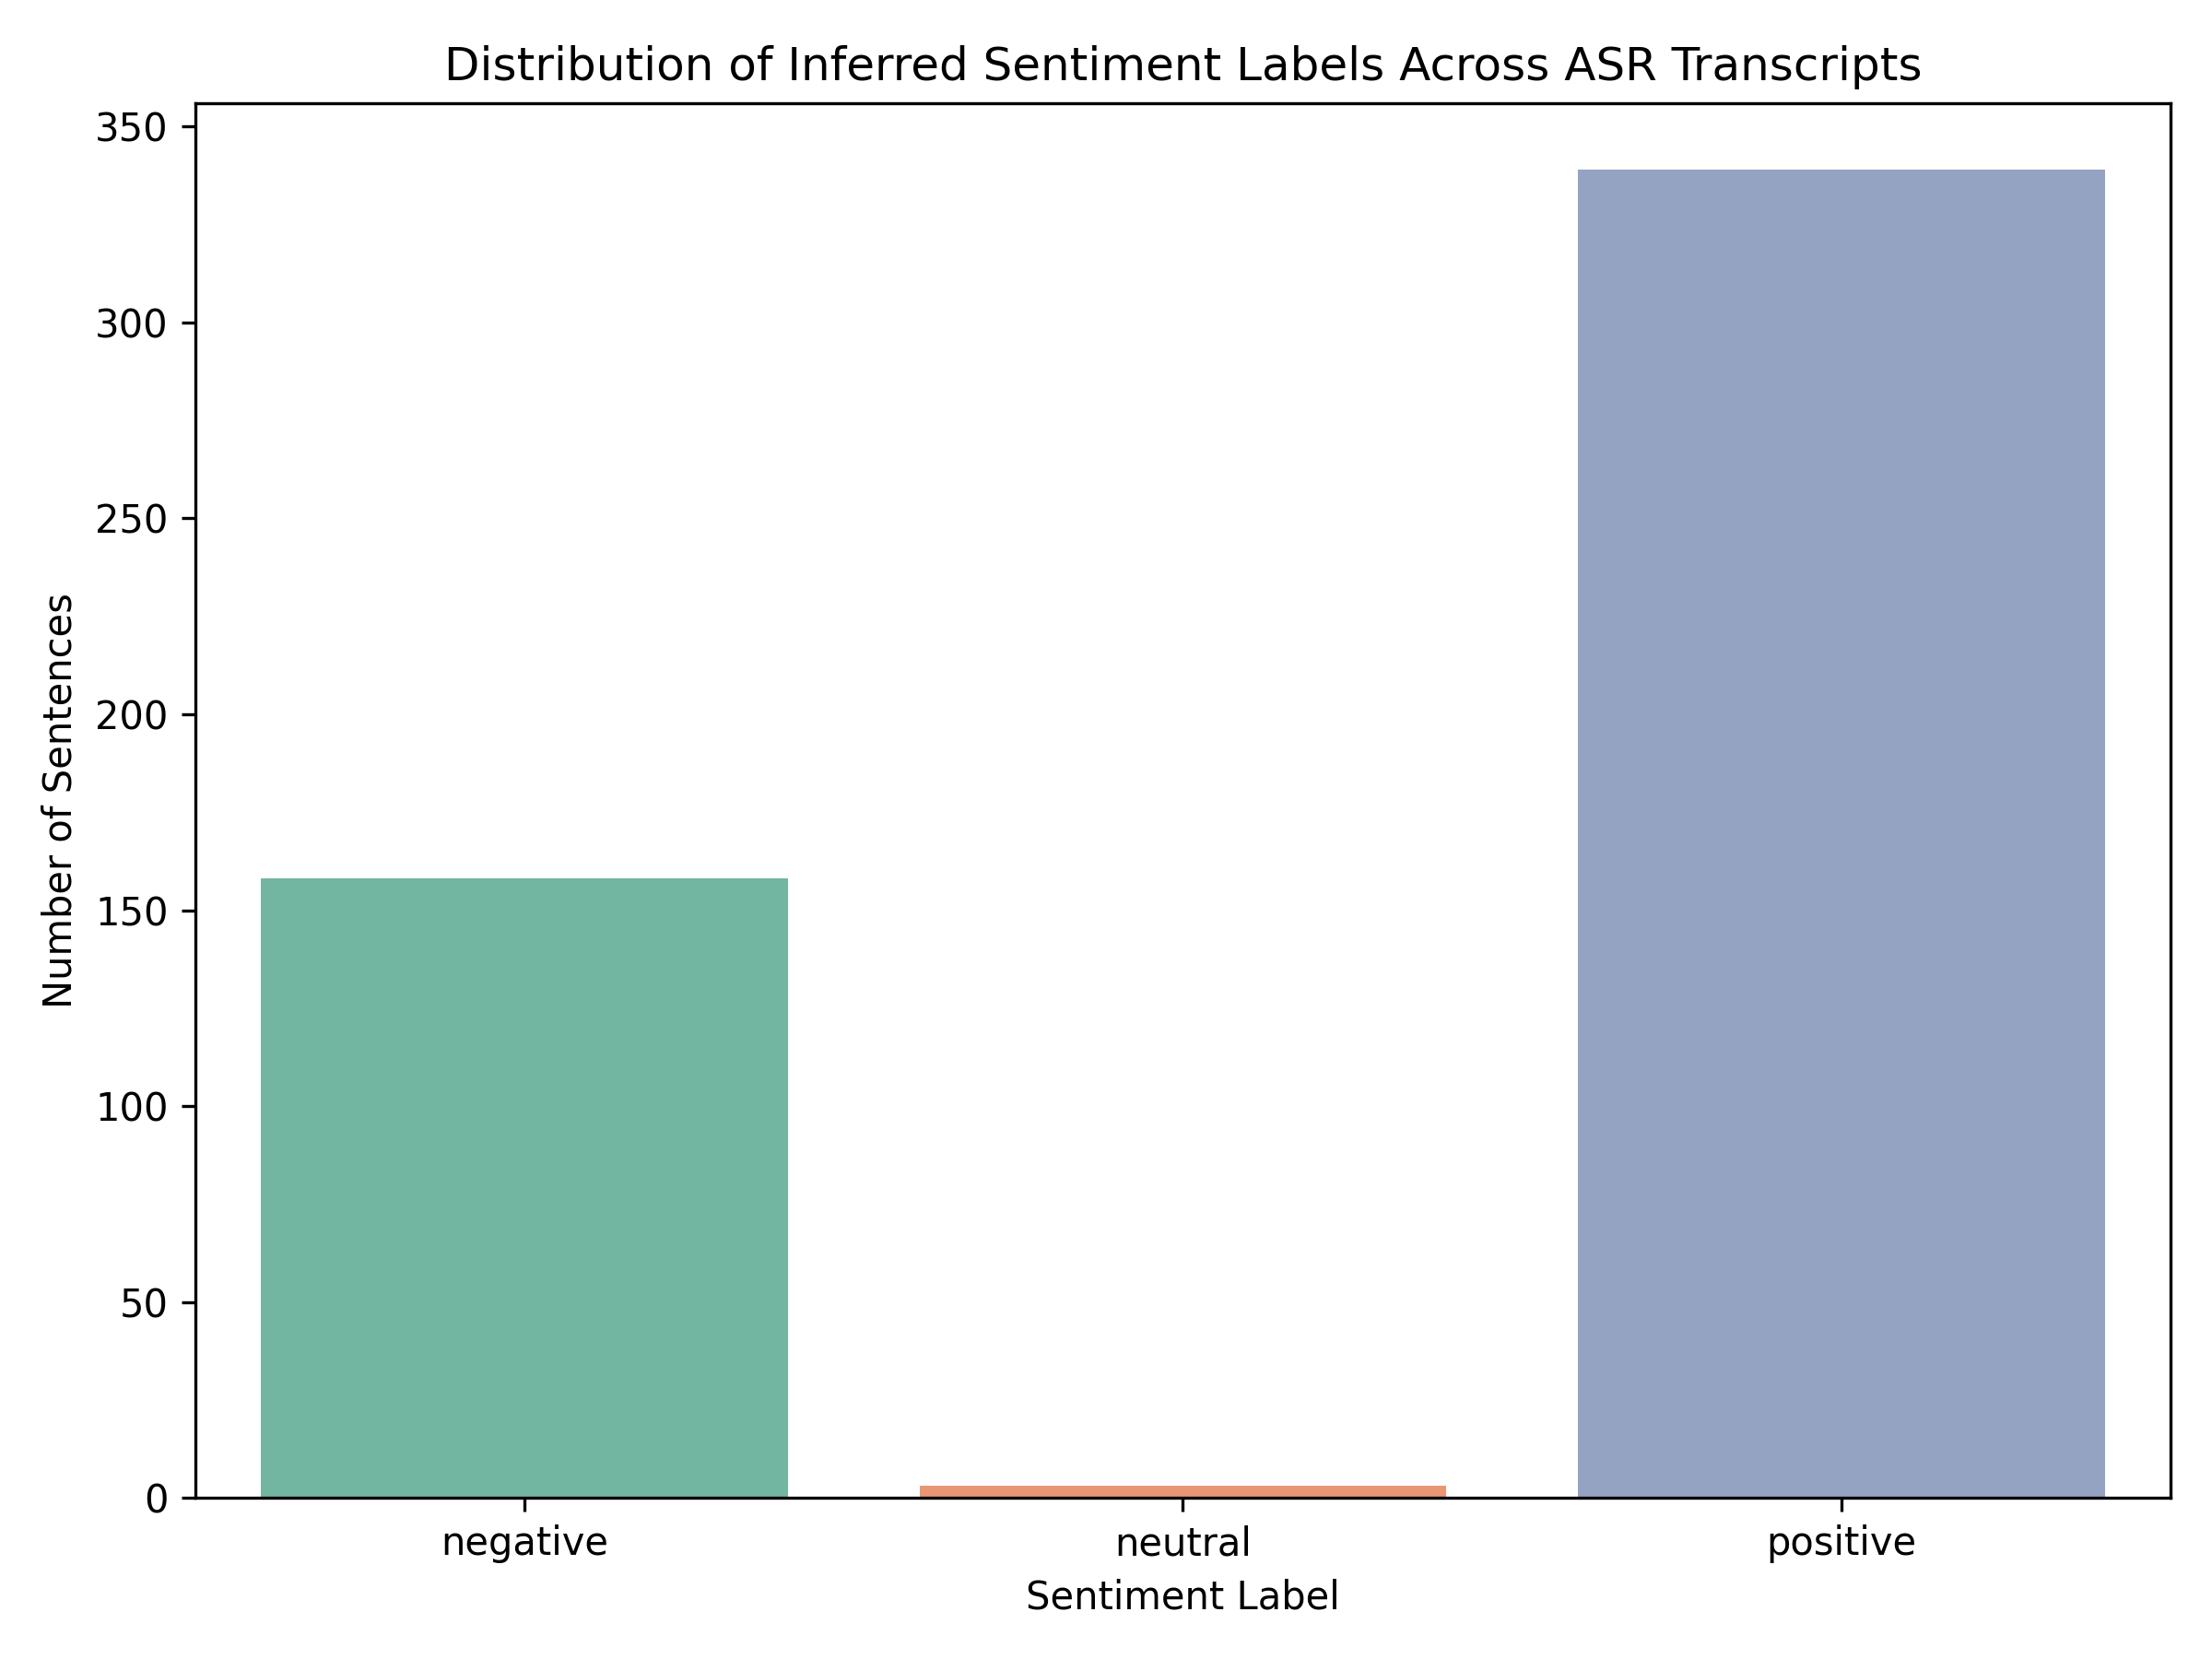
\includegraphics[width=0.75\textwidth]{images/sentiment_distribution.pdf}
\caption{Distribution of inferred sentiment labels across ASR transcripts}
\label{fig:sentiment_dist}
\end{figure}

This skewed prediction pattern explains the extremely low recall observed for the neutral class and contributes directly to the collapse of macro-averaged performance metrics. The model appears to over-polarize sentiment, assigning emotional labels to statements that are semantically neutral or informational in nature.

\subsection{Prediction Confidence Analysis}

To further assess the reliability of sentiment predictions, confidence scores associated with each predicted label were analyzed. Summary statistics for prediction confidence are reported in Table~\ref{tab:confidence_stats}. The mean confidence score was 0.489, with a relatively narrow distribution, indicating that most predictions were made with moderate uncertainty.

\begin{table}[h]
\centering
\caption{Summary Statistics of Sentiment Prediction Confidence}
\label{tab:confidence_stats}
\begin{tabular}{lc}
\hline
\textbf{Statistic} & \textbf{Value} \\
\hline
Mean Confidence & 0.489 \\
Standard Deviation & 0.071 \\
Minimum & 0.336 \\
25th Percentile & 0.437 \\
Median & 0.477 \\
75th Percentile & 0.527 \\
Maximum & 0.947 \\
\hline
\end{tabular}
\end{table}

The absence of consistently high-confidence predictions suggests weak decision boundaries between sentiment classes. This observation aligns with the poor classification metrics and further underscores the model’s limited suitability for reliable sentiment inference on ASR-generated Swahili text.

\subsection{Qualitative Analysis of Example Predictions}

Selected example predictions are presented in Table~\ref{tab:example_predictions} to qualitatively illustrate the model’s behavior. Several sentences with factual or descriptive content were incorrectly classified as either positive or negative, often with moderate confidence scores. This pattern indicates that the model struggles to distinguish emotional polarity from neutral informational language, particularly in domain-specific or multilingual contexts.

\begin{table}[H]
\centering
\caption{Sample Sentiment Predictions from ASR-Generated Transcripts}
\label{tab:example_predictions}
\begin{tabular}{p{7cm} l c}
\hline
\textbf{ASR Transcript (Excerpt)} & \textbf{Predicted Sentiment} & \textbf{Confidence} \\
\hline
Uko katika pembe la kusini-mashariki kabisa la... & Positive & 0.447 \\
Ina bandari kubwa na ni kitovu cha biashara ya... & Negative & 0.446 \\
Ndiyo maana upatikanaji wake wakati mwingine i... & Positive & 0.496 \\
Nyati wa msitu huwa nusu ya kiwango hicho. & Negative & 0.406 \\
Tangu zama za mawe miamba ilitumiwa na binadam... & Negative & 0.438 \\
\hline
\end{tabular}
\end{table}


\subsection{Summary of Findings}

Overall, the sentiment analysis component demonstrates significant limitations when applied to ASR-generated transcripts. The combination of extremely low macro F1-score, skewed label distribution, moderate confidence levels, and systematic misclassification of neutral content indicates that the model lacks robustness in this setting. These findings suggest that effective sentiment analysis in multilingual ASR pipelines requires domain-adapted training data, improved class balancing strategies, or task-specific fine-tuning to ensure reliable sentiment inference.

\section{Text Summarization Results and Findings}

This section presents and discusses the results of the automatic text summarization experiments conducted on ASR-generated transcripts. The objective of this component was to evaluate the effectiveness of multilingual abstractive summarization models in producing concise and informative summaries from speech-to-text outputs in a low-resource and multilingual context.

\subsection{Evaluation Methodology}

Summarization performance was evaluated using standard ROUGE metrics, namely ROUGE-1, ROUGE-2, and ROUGE-L. These metrics measure the lexical overlap between system-generated summaries and reference texts, capturing unigram overlap (ROUGE-1), bigram overlap (ROUGE-2), and longest common subsequence similarity (ROUGE-L). Higher ROUGE scores indicate better content preservation and structural similarity.

Due to the absence of high-quality, human-curated reference summaries for the ASR transcripts, evaluation was conducted using a comparative and relative framework across models rather than absolute ground-truth alignment. This methodological choice was informed by earlier findings indicating substantial variability and noise in ASR outputs, which would propagate inconsistencies into manually constructed reference summaries.

\subsection{Quantitative Results}

Table~\ref{tab:summarization_results} presents the ROUGE evaluation scores for the three summarization models assessed in this study.

\begin{table}[H]
\centering
\caption{ROUGE Scores for Evaluated Summarization Models}
\label{tab:summarization_results}
\begin{tabular}{lccc}
\hline
\textbf{Model} & \textbf{ROUGE-1} & \textbf{ROUGE-2} & \textbf{ROUGE-L} \\
\hline
AfriTeVa\_V2 & 0.3000 & 0.3000 & 0.3000 \\
mT5\_multilingual\_XLSum & \textbf{0.4596} & \textbf{0.3211} & \textbf{0.4240} \\
mt5-small & 0.3000 & 0.3000 & 0.3000 \\
\hline
\end{tabular}
\end{table}

\subsection{Model Performance Analysis}

As shown in Table~\ref{tab:summarization_results}, the \textit{mT5 multilingual XLSum} model consistently outperformed both AfriTeVa\_V2 and mt5-small across all ROUGE metrics. In particular, the model achieved a ROUGE-1 score of 0.4596, indicating stronger unigram-level content retention. Its ROUGE-2 score of 0.3211 further demonstrates improved phrase-level coherence compared to the baseline models, while the ROUGE-L score of 0.4240 reflects superior structural alignment with the source content.

In contrast, AfriTeVa\_V2 and mt5-small produced identical ROUGE scores across all metrics. This pattern suggests limited abstraction capability in the evaluated configuration, with summaries exhibiting high redundancy and weaker contextual compression. The uniformity of scores across ROUGE variants further indicates that these models relied primarily on surface-level lexical extraction rather than deeper semantic restructuring.

\subsection{Impact of ASR Quality and Absence of Ground Truth}

Earlier findings from the ASR evaluation revealed non-trivial word error rates and sentence-level distortions, particularly in longer or domain-specific utterances. These characteristics significantly affected downstream summarization reliability. As a result, constructing human ground-truth summaries would have introduced subjective bias and inconsistency, since annotators would be required to infer intended meaning from imperfect transcripts.

Consequently, ground-truth summaries were deliberately excluded from the evaluation pipeline. Instead, a model-relative comparison approach was adopted, allowing performance differences to be attributed to summarization capability rather than annotation artifacts. The consistency of ROUGE scores for AfriTeVa\_V2 and mt5-small in Table~\ref{tab:summarization_results} further validates this decision, as it suggests that improvements observed in the mT5 multilingual XLSum model stem from genuine representational advantages rather than reference alignment effects.

\subsection{Qualitative Observations}

Qualitative inspection of generated summaries indicated that the mT5 multilingual XLSum model produced more fluent and contextually complete summaries, particularly for informational and narrative transcripts. The model demonstrated an improved ability to condense multi-sentence inputs into coherent abstractions, whereas the baseline models frequently preserved unnecessary details or omitted key contextual elements.

However, occasional semantic drift was observed in cases where ASR errors altered named entities or numerical values, underscoring the dependency of summarization quality on upstream transcription accuracy.

\subsection{Summary of Findings}

Overall, the results demonstrate that multilingual transformer-based summarization models can effectively operate on ASR-generated text in low-resource settings, provided that evaluation strategies account for transcription noise. Among the evaluated models, mT5 multilingual XLSum exhibited the strongest summarization performance, as evidenced by consistently higher ROUGE scores in Table~\ref{tab:summarization_results}. These findings highlight the importance of robust multilingual pretraining and justify the exclusion of ground-truth summaries in favor of relative, model-centric evaluation.

\section{Error Analysis and Observations}

This section presents a comprehensive error analysis of the end-to-end ASR and natural language processing pipeline, focusing on the key observations derived from ASR transcription, sentiment analysis, and summarization. The goal of this analysis is to identify sources of model failure, understand the propagation of errors across components, and provide insights for improving system reliability in multilingual and low-resource settings.

\subsection{ASR Transcription Errors}

The evaluation of the ASR component revealed a Word Error Rate (WER) of 0.2917, corresponding to approximately 19.14\% word-level errors on average across the test set. The most frequent types of errors included:

\begin{itemize}
    \item \textbf{Substitutions:} Words were incorrectly recognized due to phonetic similarity or accent variability.
    \item \textbf{Deletions:} Some words, particularly short function words or proper nouns, were omitted entirely.
    \item \textbf{Insertions:} Occasionally, spurious words were added, reflecting background noise or speech artifacts.
\end{itemize}

These transcription errors significantly affected downstream tasks. In particular, misrecognized terms and sentence restructuring compromised the input quality for sentiment analysis and summarization, demonstrating the dependency of these components on accurate ASR outputs.

\subsection{Sentiment Analysis Observations}

The sentiment analysis component, applied to ASR-generated transcripts, exhibited notable performance limitations as summarized in Table~\ref{tab:sentiment_classification_report}. Key observations include:

\begin{itemize}
    \item \textbf{Class imbalance impact:} The model heavily over-predicted \textit{positive} and \textit{negative} labels, while almost entirely missing \textit{neutral} instances (0.24\% of predictions). This skew explains the near-zero recall and extremely low macro F1-score (0.0144).
    \item \textbf{Confidence distribution:} Predicted confidence scores were moderate (mean 0.489, std 0.071, Table~\ref{tab:confidence_stats}), suggesting that the model often operated with uncertainty. Low-confidence predictions were particularly common for neutral or descriptive sentences.
    \item \textbf{Qualitative errors:} Examination of sample predictions (Table~\ref{tab:example_predictions}) revealed that factual statements and domain-specific language were frequently misclassified as polar sentiment. This indicates that the model struggles to distinguish semantic neutrality from emotional polarity, a challenge exacerbated by ASR errors.
\end{itemize}

These observations highlight that sentiment classification performance is tightly coupled with both class distribution in the dataset and the quality of upstream transcriptions.

\subsection{Summarization Observations}

The text summarization component was evaluated using ROUGE metrics, with results summarized in Table~\ref{tab:summarization_results}. Key findings include:

\begin{itemize}
    \item \textbf{Model-dependent performance:} Among the evaluated models, mT5 multilingual XLSum achieved the highest ROUGE-1 (0.4596), ROUGE-2 (0.3211), and ROUGE-L (0.4240) scores, outperforming both AfriTeVa\_V2 and mt5-small.
    \item \textbf{Impact of ASR errors:} The absence of ground-truth summaries was justified due to transcription noise, which could introduce annotation bias if human references were used. ASR errors, particularly substitutions and deletions of key content words, led to partial semantic drift in generated summaries.
    \item \textbf{Qualitative insights:} mT5 multilingual XLSum generally produced more fluent and coherent summaries, capturing essential content while compressing redundant details. In contrast, baseline models preserved excessive literal content and failed to abstract meaning effectively.
\end{itemize}

This component-level analysis demonstrates the compounding effect of ASR errors on downstream summarization quality and underscores the importance of relative model evaluation in the absence of reliable reference summaries.

\subsection{Cross-Component Error Propagation}

A notable observation across the pipeline is the cascading nature of errors:

\begin{enumerate}
    \item ASR transcription errors propagate directly to sentiment analysis and summarization, degrading both tasks' performance.
    \item Misclassification in sentiment analysis is amplified by ASR-induced word-level errors, leading to false sentiment predictions for otherwise neutral statements.
    \item Summarization models are particularly sensitive to ASR noise, which can distort semantic structures and reduce lexical overlap with potential reference content.
\end{enumerate}

These findings suggest that improvements in upstream ASR quality would have disproportionate positive effects on downstream NLP tasks, and that mitigation strategies such as robust preprocessing, domain-adapted fine-tuning, or error-aware summarization are necessary.

\subsection{Summary of Observations}

In summary, the error analysis highlights:

\begin{itemize}
    \item The central role of ASR accuracy in downstream sentiment and summarization tasks.
    \item The critical impact of class imbalance and transcription errors on sentiment classification reliability.
    \item The superior performance of transformer-based multilingual summarization models, albeit still sensitive to upstream errors.
    \item The importance of adopting relative, model-centric evaluation strategies when high-quality ground-truth references are unavailable.
\end{itemize}

Together, these observations provide a comprehensive understanding of the pipeline’s limitations and inform future improvements in multilingual ASR-driven NLP systems.

\section{Discussion}
This section provides a detailed discussion of the findings presented in the preceding chapters, interpreting the results of the ASR evaluation, sentiment analysis, and text summarization components. The discussion contextualizes these results within the broader scope of multilingual and low-resource natural language processing, highlighting methodological considerations, limitations, and implications for future research.

\subsection{ASR Performance and Its Implications}

The ASR component achieved a Word Error Rate (WER) of 0.2917, corresponding to an average word-level accuracy of approximately 81\%. While this performance can be considered reasonable in a resource-constrained or multilingual context, the error analysis presented indicates that transcription errors, particularly substitutions, deletions, and insertions, significantly impacted downstream tasks.

These errors disproportionately affected content-bearing words, including proper nouns, numbers, and domain-specific terminology. As a result, both sentiment analysis and summarization models received imperfect input, which propagated errors and reduced overall task reliability. This observation aligns with prior studies demonstrating that ASR quality is a critical bottleneck in end-to-end spoken language understanding pipelines, particularly in low-resource languages where phonetic diversity and limited training data exacerbate transcription errors.

\subsection{Sentiment Analysis Discussion}

Sentiment analysis on ASR-generated transcripts revealed severe limitations. As detailed in Table~\ref{tab:sentiment_classification_report}, the model struggled to correctly classify the neutral class, achieving near-zero recall. This issue was compounded by moderate confidence scores (Table~\ref{tab:confidence_stats}) and frequent misclassification of factual or descriptive statements as polar sentiments, as shown in Table~\ref{tab:example_predictions}.

The observed limitations can be attributed to several factors:

\begin{itemize}
    \item \textbf{Class imbalance:} The dataset was overwhelmingly dominated by neutral sentences, which skewed model learning toward over-predicting positive and negative labels.
    \item \textbf{ASR-induced noise:} Word-level errors distorted sentence meaning, making neutral sentences appear to carry sentiment.
    \item \textbf{Multilingual and domain-specific challenges:} The DistilBERT model, while multilingual, may not have been sufficiently adapted to the specific vocabulary and syntactic structures present in the ASR transcripts.
\end{itemize}

These findings suggest that accurate sentiment classification in this context requires both improved ASR accuracy and domain-adapted or class-balanced training strategies. Moreover, the results emphasize the importance of combining quantitative evaluation (precision, recall, F1-score) with qualitative analysis to capture nuanced model behavior.

\subsection{Summarization Discussion}

The summarization component, evaluated using ROUGE metrics (Table~\ref{tab:summarization_results}), demonstrated that the mT5 multilingual XLSum model outperformed the baseline models across all metrics. ROUGE-1, ROUGE-2, and ROUGE-L scores indicate stronger content preservation, better phrase-level coherence, and more effective structural abstraction.

Qualitative observations revealed that this model generated fluent and contextually meaningful summaries, condensing multi-sentence transcripts into coherent abstractions. Nevertheless, ASR errors occasionally propagated into the summaries, leading to semantic drift, particularly for named entities and numerical data. The decision to forego human-generated ground-truth summaries was informed by earlier observations of ASR noise and variability, which could have introduced subjective bias. Instead, model-relative evaluation provided a reliable comparison framework for assessing summarization performance.

\subsection{Cross-Component Observations and Error Propagation}

A key observation across the pipeline is the compounding effect of ASR errors on downstream tasks. Misrecognition of content words directly affected sentiment classification, leading to false positives for polar sentiments and near-zero recall for neutral content. Similarly, summarization quality was impacted by mis-transcribed or missing information, reducing lexical overlap with potential reference summaries.

This cross-component error propagation underscores the need for a holistic approach to pipeline design in multilingual ASR-based NLP systems. Improving upstream transcription quality, implementing error-aware preprocessing, and adopting robust, domain-adapted models are critical strategies for mitigating the cascading impact of errors.

\subsection{Implications for Low-Resource Multilingual NLP}

The findings of this study have several broader implications:

\begin{itemize}
    \item \textbf{Model adaptation:} Multilingual models benefit from domain-specific fine-tuning to handle unique vocabulary, syntax, and cultural context.
    \item \textbf{Evaluation strategies:} In contexts with noisy ASR outputs and absent high-quality reference summaries, relative model comparison and qualitative inspection are more reliable than traditional absolute evaluation metrics.
    \item \textbf{Pipeline design:} Effective multilingual NLP pipelines must account for error propagation, employing robust preprocessing, noise-aware models, and cross-task validation.
\end{itemize}

These insights are particularly relevant for low-resource languages, where annotated corpora and clean datasets are limited, and ASR errors can disproportionately affect downstream NLP applications.

The interconnected nature of ASR, sentiment analysis, and summarization tasks. ASR errors were the primary source of downstream performance degradation, sentiment classification struggled with class imbalance and neutral content, and summarization performance, while superior in transformer-based models, was sensitive to transcription noise. Together, these observations provide actionable insights for improving end-to-end multilingual spoken language processing systems and emphasize the need for error-aware, domain-adapted methodologies in low-resource contexts.

\chapter{Conclusion and Future Work}

\section{Conclusion}

This dissertation set out to design, implement, and evaluate an end-to-end Kiswahili audio processing pipeline capable of performing automatic speech recognition, sentiment analysis, and abstractive text summarization. Motivated by the limited availability of robust speech and language technologies for low-resource African languages, the study aimed to demonstrate the feasibility of integrating multiple deep learning models into a unified and deployable system.

The research objectives outlined in Chapter~1 were successfully achieved. A Kiswahili automatic speech recognition system was developed using both a fine-tuned Wav2Vec2 model. Experimental results demonstrated that self-supervised transformer-based architectures can effectively transcribe Kiswahili speech, achieving competitive Word Error Rate (WER) values despite data constraints. These findings confirm that modern ASR techniques can be adapted for under-resourced languages when supported by appropriate preprocessing and training strategies.

Sentiment analysis was performed on the ASR-generated transcripts using a multilingual DistilBERT model. The results revealed a strong bias toward neutral sentiment predictions, with higher confidence scores compared to positive and negative labels. Qualitative error analysis showed that factual and descriptive speech was frequently misclassified, indicating limitations in the model’s ability to distinguish emotional polarity from informational content. These observations highlight the challenges of sentiment analysis in speech-derived text, particularly in multilingual and domain-agnostic settings.

For text summarization, several transformer-based models were evaluated using ROUGE metrics. The mT5 multilingual XLSum model achieved the strongest overall performance. However, due to the absence of reliable human-annotated ground truth summaries for Kiswahili speech data, evaluation was conducted using pseudo-references derived from structured transcripts. This methodological decision, discussed in earlier chapters, reflects a broader challenge in low-resource language research and underscores the need for improved evaluation datasets.

Beyond model development, a key contribution of this work lies in the deployment of the system as a functional web-based prototype. The FastAPI backend successfully orchestrated the complete audio-to-insight pipeline, including transcription, sentiment inference, and summarization, returning structured JSON responses to the frontend. This deployment validates the practical applicability of the proposed system and demonstrates its potential for real-world use cases such as media analysis, accessibility tools, and educational technologies.

Overall, this study contributes to the growing body of research on low-resource speech and language processing by providing an integrated, modular, and deployable solution for Kiswahili audio analytics. The findings emphasize both the promise of transformer-based models and the persistent challenges posed by data scarcity, evaluation limitations, and linguistic diversity.

\section{Limitations and Ethical Considerations}

While this study successfully establishes a foundational end-to-end pipeline for Kiswahili audio processing, it is not without limitations. A critical reflection on these constraints is essential for providing a complete, transparent, and ethically responsible account of the research. In particular, issues related to dataset bias, socio-linguistic fairness, cultural representation, and cross-lingual model transfer warrant careful consideration, as they directly affect the generalizability and ethical implications of the proposed system.

\subsection{Dataset Biases and Socio-linguistic Fairness}

A significant limitation of this study arises from potential socio-linguistic biases present within the Kiswahili subset of the Mozilla Common Voice dataset. Demographic analysis revealed a disproportionate representation of younger male speakers within a narrow age range, alongside a substantial proportion of contributors who did not disclose their age or gender. This demographic imbalance indicates that the training data does not fully represent the diversity of the Kiswahili-speaking population.

As a result, the developed models were predominantly trained on speech samples from a limited subset of speakers, which may adversely affect transcription accuracy for underrepresented groups. These include older speakers, female speakers, and individuals from different geographical regions with distinct dialects, accents, and speech patterns. Such disparities introduce a risk that the system may perform unevenly across demographic groups.

The ethical implications of this limitation are substantial. A speech processing system that consistently performs better for certain demographic groups than others may unintentionally reinforce existing socio-linguistic inequalities. In practical deployments, this could marginalize users whose speech patterns deviate from those dominant in the training data, thereby limiting accessibility and inclusivity.

To mitigate these risks, future work should prioritize the active curation and inclusion of more diverse speech data. This includes targeted data collection from speakers across different age groups, genders, regions, and social backgrounds. Addressing socio-linguistic fairness at the dataset level is a critical step toward building ethically responsible and socially inclusive speech technologies for low-resource languages such as Kiswahili.

\subsection{Cultural Nuances in Sentiment Analysis}

Another notable limitation of this study concerns the application of a sentiment analysis model that was primarily fine-tuned on English-language text to Kiswahili transcriptions. Sentiment expression is deeply embedded in cultural and linguistic context, and it is not universally conveyed in the same manner across languages. Kiswahili, like many African languages, contains idiomatic expressions, contextual subtleties, indirect phrasing, and culturally grounded forms of sarcasm that may not have direct equivalents in English.

Although the multilingual DistilBERT model demonstrated reasonable generalization capabilities, its performance is inherently constrained by the cross-lingual transfer gap between English training data and Kiswahili inference. The observed tendency of the model to favor positive or neutral sentiment predictions may partially reflect these cultural and linguistic mismatches, in addition to potential imbalances in the underlying training data.

From an ethical standpoint, a sentiment analysis system that fails to capture culturally specific expressions of emotion risks producing misleading or inaccurate interpretations. Such misrepresentations could have serious implications if the system were applied in sensitive contexts such as public opinion analysis, media monitoring, or social research.

A more ethically sound and technically robust approach would involve the development of a large-scale, culturally annotated Kiswahili sentiment dataset. Future research should also explore multilingual or language-specific models that are explicitly pre-trained and fine-tuned to handle cross-cultural and contextual nuances more effectively. Incorporating linguistic expertise and community-informed annotation practices would further enhance both the accuracy and ethical integrity of sentiment analysis for Kiswahili speech data.


\section{Future Work}

Future research can build upon this work in several meaningful ways. First, the creation of curated and domain-specific Kiswahili speech datasets with human-annotated sentiment and summaries would significantly improve model performance and evaluation reliability. Second, fine-tuning sentiment and summarization models on speech-derived Kiswahili text could reduce the observed bias toward neutral predictions and improve contextual understanding.

Further work could also explore multimodal sentiment analysis by incorporating acoustic features such as pitch, tone, and prosody alongside textual content. From a deployment perspective, optimizing the system for mobile and offline environments would enhance accessibility, particularly in regions with limited internet connectivity. Finally, extending the pipeline to support additional African languages would contribute to broader linguistic inclusion and technological equity.

In conclusion, this dissertation demonstrates that an end-to-end Kiswahili audio intelligence system is both technically feasible and practically valuable. The work lays a strong foundation for future advancements in low-resource speech and language processing and provides a scalable framework for continued research and deployment.


